%Autor: Simon Walker
%Version: 1.0
%Datum: 11.12.2019
%Lizenz: CC BY-NC-SA

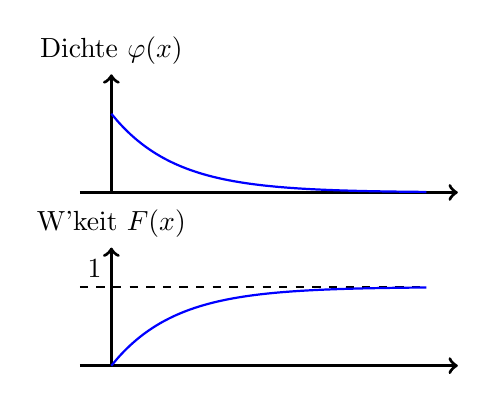
\begin{tikzpicture}[xscale=0.8, yscale=1]
	\def\a{1}
	\def\yOf{2.2} %Y Offsent
	\def\xMax{5}
	
	%Dichte funktion
	%Achsen
	\draw[very thick, ->] (-0.5, \yOf) -- (\xMax+0.5, \yOf);
	\draw[very thick, ->] (0, \yOf) -- (0, \yOf + \a +0.5);
	\node[above] at (0, \yOf + \a +0.5) {Dichte $\varphi(x)$};
	
	\draw[blue, thick]
	plot[smooth, samples=50, variable=\x, domain=0:\xMax]
	(\x, {\a * exp(\a*\x*-1)+\yOf});
	
	%Verteilungsfunktion
	%Achsen
	\draw[very thick, ->] (-0.5, 0) -- (\xMax+0.5, 0);
	\draw[very thick, ->] (0, 0) -- (0, 1.5);
	\node[above] at (0, 1.5) {W'keit $F(x)$};
	
	\draw[dashed] (-0.5, 1) -- (\xMax, 1);
	\node[above left] at (0, 1) {$1$};
	
	\draw[blue, thick]
	plot[smooth, samples=50, variable=\x, domain=0:\xMax]
	(\x, {1- (exp(\a*\x*-1))});
	
\end{tikzpicture}
